
%% bare_conf.tex
%% V1.3
%% 2007/01/11
%% by Michael Shell
%% See:
%% http://www.michaelshell.org/
%% for current contact information.
%%
%% This is a skeleton file demonstrating the use of IEEEtran.cls
%% (requires IEEEtran.cls version 1.7 or later) with an IEEE conference paper.
%%
%% Support sites:
%% http://www.michaelshell.org/tex/ieeetran/
%% http://www.ctan.org/tex-archive/macros/latex/contrib/IEEEtran/
%% and
%% http://www.ieee.org/

%%*************************************************************************
%% Legal Notice:
%% This code is offered as-is without any warranty either expressed or
%% implied; without even the implied warranty of MERCHANTABILITY or
%% FITNESS FOR A PARTICULAR PURPOSE! 
%% User assumes all risk.
%% In no event shall IEEE or any contributor to this code be liable for
%% any damages or losses, including, but not limited to, incidental,
%% consequential, or any other damages, resulting from the use or misuse
%% of any information contained here.
%%
%% All comments are the opinions of their respective authors and are not
%% necessarily endorsed by the IEEE.
%%
%% This work is distributed under the LaTeX Project Public License (LPPL)
%% ( http://www.latex-project.org/ ) version 1.3, and may be freely used,
%% distributed and modified. A copy of the LPPL, version 1.3, is included
%% in the base LaTeX documentation of all distributions of LaTeX released
%% 2003/12/01 or later.
%% Retain all contribution notices and credits.
%% ** Modified files should be clearly indicated as such, including  **
%% ** renaming them and changing author support contact information. **
%%
%% File list of work: IEEEtran.cls, IEEEtran_HOWTO.pdf, bare_adv.tex,
%%                    bare_conf.tex, bare_jrnl.tex, bare_jrnl_compsoc.tex
%%*************************************************************************

% *** Authors should verify (and, if needed, correct) their LaTeX system  ***
% *** with the testflow diagnostic prior to trusting their LaTeX platform ***
% *** with production work. IEEE's font choices can trigger bugs that do  ***
% *** not appear when using other class files.                            ***
% The testflow support page is at:
% http://www.michaelshell.org/tex/testflow/



% Note that the a4paper option is mainly intended so that authors in
% countries using A4 can easily print to A4 and see how their papers will
% look in print - the typesetting of the document will not typically be
% affected with changes in paper size (but the bottom and side margins will).
% Use the testflow package mentioned above to verify correct handling of
% both paper sizes by the user's LaTeX system.
%
% Also note that the "draftcls" or "draftclsnofoot", not "draft", option
% should be used if it is desired that the figures are to be displayed in
% draft mode.
%
\documentclass[draftclsnofoot]{elsarticle}
% Add the compsoc option for Computer Society conferences.
%
% If IEEEtran.cls has not been installed into the LaTeX system files,
% manually specify the path to it like:
% \documentclass[conference]{../sty/IEEEtran}





% Some very useful LaTeX packages include:
% (uncomment the ones you want to load)


% *** MISC UTILITY PACKAGES ***
%
%\usepackage{ifpdf}
% Heiko Oberdiek's ifpdf.sty is very useful if you need conditional
% compilation based on whether the output is pdf or dvi.
% usage:
% \ifpdf
%   % pdf code
% \else
%   % dvi code
% \fi
% The latest version of ifpdf.sty can be obtained from:
% http://www.ctan.org/tex-archive/macros/latex/contrib/oberdiek/
% Also, note that IEEEtran.cls V1.7 and later provides a builtin
% \ifCLASSINFOpdf conditional that works the same way.
% When switching from latex to pdflatex and vice-versa, the compiler may
% have to be run twice to clear warning/error messages.






% *** CITATION PACKAGES ***
%
%\usepackage{cite}
% cite.sty was written by Donald Arseneau
% V1.6 and later of IEEEtran pre-defines the format of the cite.sty package
% \cite{} output to follow that of IEEE. Loading the cite package will
% result in citation numbers being automatically sorted and properly
% "compressed/ranged". e.g., [1], [9], [2], [7], [5], [6] without using
% cite.sty will become [1], [2], [5]--[7], [9] using cite.sty. cite.sty's
% \cite will automatically add leading space, if needed. Use cite.sty's
% noadjust option (cite.sty V3.8 and later) if you want to turn this off.
% cite.sty is already installed on most LaTeX systems. Be sure and use
% version 4.0 (2003-05-27) and later if using hyperref.sty. cite.sty does
% not currently provide for hyperlinked citations.
% The latest version can be obtained at:
% http://www.ctan.org/tex-archive/macros/latex/contrib/cite/
% The documentation is contained in the cite.sty file itself.






% *** GRAPHICS RELATED PACKAGES ***
%
   %\usepackage[pdftex]{graphicx}
  % declare the path(s) where your graphic files are
  \graphicspath{{imgs/}}
  % and their extensions so you won't have to specify these with
  % every instance of \includegraphics
% installed on most LaTeX systems. The latest version and documentation can
% be obtained at: 
% http://www.ctan.org/tex-archive/macros/latex/required/graphics/
% Another good source of documentation is "Using Imported Graphics in
% LaTeX2e" by Keith Reckdahl which can be found as epslatex.ps or
% epslatex.pdf at: http://www.ctan.org/tex-archive/info/
%
% latex, and pdflatex in dvi mode, support graphics in encapsulated
% postscript (.eps) format. pdflatex in pdf mode supports graphics
% in .pdf, .jpeg, .png and .mps (metapost) formats. Users should ensure
% that all non-photo figures use a vector format (.eps, .pdf, .mps) and
% not a bitmapped formats (.jpeg, .png). IEEE frowns on bitmapped formats
% which can result in "jaggedy"/blurry rendering of lines and letters as
% well as large increases in file sizes.
%
% You can find documentation about the pdfTeX application at:
% http://www.tug.org/applications/pdftex





% *** MATH PACKAGES ***
%
%\usepackage[cmex10]{amsmath}
% A popular package from the American Mathematical Society that provides
% many useful and powerful commands for dealing with mathematics. If using
% it, be sure to load this package with the cmex10 option to ensure that
% only type 1 fonts will utilized at all point sizes. Without this option,
% it is possible that some math symbols, particularly those within
% footnotes, will be rendered in bitmap form which will result in a
% document that can not be IEEE Xplore compliant!
%
% Also, note that the amsmath package sets \interdisplaylinepenalty to 10000
% thus preventing page breaks from occurring within multiline equations. Use:
%\interdisplaylinepenalty=2500
% after loading amsmath to restore such page breaks as IEEEtran.cls normally
% does. amsmath.sty is already installed on most LaTeX systems. The latest
% version and documentation can be obtained at:
% http://www.ctan.org/tex-archive/macros/latex/required/amslatex/math/





% *** SPECIALIZED LIST PACKAGES ***
%
%\usepackage{algorithmic}
% algorithmic.sty was written by Peter Williams and Rogerio Brito.
% This package provides an algorithmic environment fo describing algorithms.
% You can use the algorithmic environment in-text or within a figure
% environment to provide for a floating algorithm. Do NOT use the algorithm
% floating environment provided by algorithm.sty (by the same authors) or
% algorithm2e.sty (by Christophe Fiorio) as IEEE does not use dedicated
% algorithm float types and packages that provide these will not provide
% correct IEEE style captions. The latest version and documentation of
% algorithmic.sty can be obtained at:
% http://www.ctan.org/tex-archive/macros/latex/contrib/algorithms/
% There is also a support site at:
% http://algorithms.berlios.de/index.html
% Also of interest may be the (relatively newer and more customizable)
% algorithmicx.sty package by Szasz Janos:
% http://www.ctan.org/tex-archive/macros/latex/contrib/algorithmicx/




% *** ALIGNMENT PACKAGES ***
%
%\usepackage{array}
% Frank Mittelbach's and David Carlisle's array.sty patches and improves
% the standard LaTeX2e array and tabular environments to provide better
% appearance and additional user controls. As the default LaTeX2e table
% generation code is lacking to the point of almost being broken with
% respect to the quality of the end results, all users are strongly
% advised to use an enhanced (at the very least that provided by array.sty)
% set of table tools. array.sty is already installed on most systems. The
% latest version and documentation can be obtained at:
% http://www.ctan.org/tex-archive/macros/latex/required/tools/


%\usepackage{mdwmath}
%\usepackage{mdwtab}
% Also highly recommended is Mark Wooding's extremely powerful MDW tools,
% especially mdwmath.sty and mdwtab.sty which are used to format equations
% and tables, respectively. The MDWtools set is already installed on most
% LaTeX systems. The lastest version and documentation is available at:
% http://www.ctan.org/tex-archive/macros/latex/contrib/mdwtools/


% IEEEtran contains the IEEEeqnarray family of commands that can be used to
% generate multiline equations as well as matrices, tables, etc., of high
% quality.


%\usepackage{eqparbox}
% Also of notable interest is Scott Pakin's eqparbox package for creating
% (automatically sized) equal width boxes - aka "natural width parboxes".
% Available at:
% http://www.ctan.org/tex-archive/macros/latex/contrib/eqparbox/





% *** SUBFIGURE PACKAGES ***
\usepackage[tight,footnotesize]{subfigure}
\usepackage{multirow}
% subfigure.sty was written by Steven Douglas Cochran. This package makes it
% easy to put subfigures in your figures. e.g., "Figure 1a and 1b". For IEEE
% work, it is a good idea to load it with the tight package option to reduce
% the amount of white space around the subfigures. subfigure.sty is already
% installed on most LaTeX systems. The latest version and documentation can
% be obtained at:
% http://www.ctan.org/tex-archive/obsolete/macros/latex/contrib/subfigure/
% subfigure.sty has been superceeded by subfig.sty.



%\usepackage[caption=false]{caption}
%\usepackage[font=footnotesize]{subfig}
% subfig.sty, also written by Steven Douglas Cochran, is the modern
% replacement for subfigure.sty. However, subfig.sty requires and
% automatically loads Axel Sommerfeldt's caption.sty which will override
% IEEEtran.cls handling of captions and this will result in nonIEEE style
% figure/table captions. To prevent this problem, be sure and preload
% caption.sty with its "caption=false" package option. This is will preserve
% IEEEtran.cls handing of captions. Version 1.3 (2005/06/28) and later 
% (recommended due to many improvements over 1.2) of subfig.sty supports
% the caption=false option directly:
%\usepackage[caption=false,font=footnotesize]{subfig}
%
% The latest version and documentation can be obtained at:
% http://www.ctan.org/tex-archive/macros/latex/contrib/subfig/
% The latest version and documentation of caption.sty can be obtained at:
% http://www.ctan.org/tex-archive/macros/latex/contrib/caption/




% *** FLOAT PACKAGES ***
%
%\usepackage{fixltx2e}
% fixltx2e, the successor to the earlier fix2col.sty, was written by
% Frank Mittelbach and David Carlisle. This package corrects a few problems
% in the LaTeX2e kernel, the most notable of which is that in current
% LaTeX2e releases, the ordering of single and double column floats is not
% guaranteed to be preserved. Thus, an unpatched LaTeX2e can allow a
% single column figure to be placed prior to an earlier double column
% figure. The latest version and documentation can be found at:
% http://www.ctan.org/tex-archive/macros/latex/base/



%\usepackage{stfloats}
% stfloats.sty was written by Sigitas Tolusis. This package gives LaTeX2e
% the ability to do double column floats at the bottom of the page as well
% as the top. (e.g., "\begin{figure*}[!b]" is not normally possible in
% LaTeX2e). It also provides a command:
%\fnbelowfloat
% to enable the placement of footnotes below bottom floats (the standard
% LaTeX2e kernel puts them above bottom floats). This is an invasive package
% which rewrites many portions of the LaTeX2e float routines. It may not work
% with other packages that modify the LaTeX2e float routines. The latest
% version and documentation can be obtained at:
% http://www.ctan.org/tex-archive/macros/latex/contrib/sttools/
% Documentation is contained in the stfloats.sty comments as well as in the
% presfull.pdf file. Do not use the stfloats baselinefloat ability as IEEE
% does not allow \baselineskip to stretch. Authors submitting work to the
% IEEE should note that IEEE rarely uses double column equations and
% that authors should try to avoid such use. Do not be tempted to use the
% cuted.sty or midfloat.sty packages (also by Sigitas Tolusis) as IEEE does
% not format its papers in such ways.





% *** PDF, URL AND HYPERLINK PACKAGES ***
%
\usepackage{url}
% url.sty was written by Donald Arseneau. It provides better support for
% handling and breaking URLs. url.sty is already installed on most LaTeX
% systems. The latest version can be obtained at:
% http://www.ctan.org/tex-archive/macros/latex/contrib/misc/
% Read the url.sty source comments for usage information. Basically,
% \url{my_url_here}.





% *** Do not adjust lengths that control margins, column widths, etc. ***
% *** Do not use packages that alter fonts (such as pslatex).         ***
% There should be no need to do such things with IEEEtran.cls V1.6 and later.
% (Unless specifically asked to do so by the journal or conference you plan
% to submit to, of course. )


% correct bad hyphenation here
\hyphenation{op-tical net-works semi-conduc-tor}
\usepackage{AMMALanguages,textcomp,upquote}
\usepackage{listings}
\usepackage{amsmath}
\usepackage{amsfonts}


\lstdefinelanguage{PNB}{
        morekeywords={kernel,in,vector,scalar,constant,read, write, endkernel,generate},
        morekeywords={\#pragma,\#ifdef },
        emph={CUDA, SUM,ACCURATE,MPI, OCL, OMP, AVERAGE, FAST},
        sensitive=true,
        morecomment=[l]{//},
        morestring=[b]"
}

\journal{Journal of Computer and System Sciences}
\begin{document}
\begin{frontmatter}
%
% paper title
% can use linebreaks \\ within to get better formatting as desired
\title{PNBsolver: A Domain-Specific Language for Modeling Parallel N-body Problems
%PNBsolver: A Case Study on \\Modeling Parallel N-body Programs
}




% author names and affiliations
% use a multiple column layout for up to three different
% affiliations
\author{Ferosh Jacob$^*$, Md Ashfakul Islam}
\ead{fjacob@crimson.ua.edu, mislam@crimson.ua.edu}
\address{Department of Computer Science, University of Alabama}
\cortext[cor1]{Corresponding author}

\author{Weihua Geng}
\ead{wgeng@as.ua.edu}
\address{Department of Mathematics, University of Alabama}

\author{Jeff Gray, Susan Vrbsky, Brandon Dixon}
\ead{gray@cs.ua.edu, vrbsky@cs.ua.edu, dixon@cs.ua.edu}
\address{Department of Computer Science, University of Alabama}

\author{Purushotham Bangalore}
\ead{puri@cis.uab.edu}
\address{Computer and Information Sciences,University of Alabama at Birmingham}
%}
%\IEEEauthorblockA{\IEEEauthorrefmark{1}Department of Computer Science,
%University of Alabama\\
%Email: \{fjacob, mislam\}@crimson.ua.edu, \{gray, dixon, vrbsky\}@cs.ua.edu}
%\IEEEauthorblockA{\IEEEauthorrefmark{2}Department of Mathematics,
%University of Alabama,
%Email: wgeng@as.ua.edu}
%\IEEEauthorblockA{\IEEEauthorrefmark{3}
%Email: puri@cis.uab.edu}
%
%}
% conference papers do not typically use \thanks and this command
% is locked out in conference mode. If really needed, such as for
% the acknowledgment of grants, issue a \IEEEoverridecommandlockouts
% after \documentclass

% for over three affiliations, or if they all won't fit within the width
% of the page, use this alternative format:
% 
%Homer Simpson\IEEEauthorrefmark{2},
%James Kirk\IEEEauthorrefmark{3}, 
%Montgomery Scott\IEEEauthorrefmark{3} and
%Eldon Tyrell\IEEEauthorrefmark{4}}
%\IEEEauthorblockA{\IEEEauthorrefmark{1}School of Electrical and Computer Engineering\\
%Georgia Institute of Technology,
%Atlanta, Georgia 30332--0250\\ Email: see http://www.michaelshell.org/contact.html}
%\IEEEauthorblockA{\IEEEauthorrefmark{2}Twentieth Century Fox, Springfield, USA\\
%Email: homer@thesimpsons.com}
%\IEEEauthorblockA{\IEEEauthorrefmark{3}Starfleet Academy, San Francisco, California 96678-2391\\
%Telephone: (800) 555--1212, Fax: (888) 555--1212}
%\IEEEauthorblockA{\IEEEauthorrefmark{4}Tyrell Inc., 123 Replicant Street, Los Angeles, California 90210--4321}}




% use for special paper notices
%\IEEEspecialpapernotice{(Invited Paper)}




% make the title area

\begin{abstract}
With the advent of multicore processors, parallel computation has become a necessity for next generation applications. It  is often a tedious task for domain users
to optimize their programs for a specific platform, algorithm, and problem size. We believe that domain users should be freed from this task and they should be equipped
with tool support to  reuse the optimized solutions written by expert parallel programmers. In this paper,  we introduce a two-stage modeling approach
that allows domain users to express the problem using domain constructs and reuse the available optimized solutions. This approach has been applied successfully to N-body problems using  
a domain-specific language called PNBsolver, which allows domain users to specify the  computations in an N-body problem without any implementation or platform-specific details.  
Using the PNBsolver, the domain users are allowed to control the platform and implementation of the generated code. The accuracy and execution time of the generated code can also be 
fine-tuned based on the parameters provided in PNBsolver.  We also show how common N-body interactions are implemented using PNBSolver. 
\end{abstract}
%\begin{keyword}
%% keywords here, in the form: keyword \sep keyword

%% MSC codes here, in the form: \MSC code \sep code
%% or \MSC[2008] code \sep code (2000 is the default)

%\end{keyword}
\end{frontmatter}
% IEEEtran.cls defaults to using nonbold math in the Abstract.
% This preserves the distinction between vectors and scalars. However,
% if the conference you are submitting to favors bold math in the abstract,
% then you can use LaTeX's standard command \boldmath at the very start
% of the abstract to achieve this. Many IEEE journals/conferences frown on
% math in the abstract anyway.

% no keywords




% For peer review papers, you can put extra information on the cover
% page as needed:
% \ifCLASSOPTIONpeerreview
% \begin{center} \bfseries EDICS Category: 3-BBND \end{center}
% \fi
%
% For peerreview papers, this IEEEtran command inserts a page break and
% creates the second title. It will be ignored for other modes.
%\IEEEpeerreviewmaketitle




% anywhere on the first page for that matter. Also, in-text middle ("here")
% positioning is not used. Most IEEE journals/conferences use top floats
% exclusively. Note that, LaTeX2e, unlike IEEE journals/conferences, places
% footnotes above bottom floats. This can be corrected via the \fnbelowfloat
% command of the stfloats package.

\section{Introduction} 
Even though the first computing machine built by Charles Babbage  is believed to be a parallel machine \cite{babage}, until the last few years parallel
computing was reserved for the scientific community. Recently, parallel programming has emerged as an essential skill for software developers, primarily due to
two reasons: 1) As the chip industry hit the power wall, manufactures shifted to chip multiprocessors  (CMPs), and 2) Introduction of 
Graphical Processing Units (GPUs) for general-purpose computation (GPGPU) \cite{gpgpu}.  To utilize the increased computation power available in desktops 
and powerful GPUs, parallel computing is an essential skill for the next generation of software engineers.
Because of the nature of parallel applications, programmers will have to adapt to a new style of programming to use the resources, as well as to maintain and evolve
for future applications \cite{comparison}.

Popular parallel programming paradigms include: 1) OpenMP \cite{openmp} (Shared memory), 2) Message Passing Interface\footnote{MPI, 
\url{http://www.open-mpi.org/}} (Distributed memory), and 3) CUDA\footnote{CUDA, \url{http://developer.nvidia.com/category/zone/cuda-zone}} and 
OpenCL\footnote{OpenCL, \url{http://www.khronos.org/opencl/}} for GPU platforms. All of these parallel programming paradigms have their advantages and disadvantages
for a given problem, based on the execution environment, implementation, and even size of the problem.  
In the current scenario, to find the optimized execution time for a problem of a given size in a specific platform, a programmer must manually write a parallel version, 
optimize it and compare the execution time with other platforms. It is often hard for programmers to optimize these programs because their domain of expertise is the problem domain
and not the High Performance Computing (HPC) domain. To solve this problem, programmers should be freed from implementation and optimization of parallel versions, but should have
the flexibility to express the problem and switch between execution environments (optimal execution time is also a function of problem size). There is 
no magical tool to convert any sequential program to an optimized parallel program. However, for a restricted domain this can be achieved \cite{liszt,trilinos,spiral}. In this paper, 
we address two research questions that are summarized in the following subsections.

\subsection{Q1: Separating specification and implementation}
\label{sec_q1}
Which algorithm on a specific platform can provide the optimized execution for a problem of fixed size?
To answer this question, the best way is to  develop and execute programs  implementing various algorithms in that platform for a fixed size. This leads to the task of rewriting thousands 
of lines of code. Can we reuse the implementation for another similar problem? This is possible only if the implementation details are separated from the problem specification.
Is there a better algorithm which can give the optimized execution for the specific-problem? This cannot be
linked with the existing code even if the problem specification is separated from the implementation. 

\subsection{Q2: Abstract problem specification} 
\label{sec_q2}
How can we maintain and switch between many program versions to provide the optimized execution time?
As mentioned earlier, there can be many implementations for a given problem specification. If all such implementations are based on an abstract problem specification, any of these
implementations can be used with the given problem specification. If the domain is limited, we can provide optimized solutions in required platforms for each of these implementations.

We used modeling techniques from software engineering to provide separation of specification and implementation and abstraction in a restricted domain. Our solution approach is
explained in the following subsection.  

\subsection{Solution approach: Modeling parallel programs}
 

Models in the context of software modeling can be defined as the abstract representation of a system. Model-driven Engineering \cite{modeldriven} is a methodology that makes use 
of a Domain-Specific Modeling Language (DSML) \cite{ds1,dsml} such that it can: 1) define a system using domain information, 2) analyze the domain, and 3) automatically generate  
source code or other artifacts by code generation techniques. A model is defined by a set of 
entities, associations and constraints, commonly called a metamodel \cite{modeldriven1}. In the case of a Domain-Specific Language (DSL) \cite{dsl}, a metamodel is the grammar defining 
the DSL. The domain experts define domain problems in a DSL file (an instance of the model), which is capable of capturing information to represent the whole system.

We developed a two-stage technique for modeling parallel programs. In the first stage, the domain experts create a model (DSL file) specifying 
the problem (this model has no platform-specific or implementation-specific details) and in the second stage,  this model is mapped to different platforms and implementations
 based on user preferences. The main advantage of this two-step modeling technique is that it can be extended to include additional platforms and implementations and is well-suited
 for a domain like parallel programming.

In this paper, we introduce PNBsolver, which is a DSL based on our two-stage modeling technique. PNBsolver can represent
N-body problems without any implementation details and also has the flexibility to allow users to switch between implementations (algorithms) and platforms. 
Section \ref{analysis} overviews N-body problems and analyzes a commonly used algorithm in such problems. Section \ref{working} describes PNBsolver from a user's perspective
and the implementation details are explained in Section \ref{implementation}. Section \ref{sec_cmp} gives details of a comparison study of PNBsolver solutions with existing
implementations. Additional examples using PNBsolver are shown in Section \ref{sec_more}. Related works are reviewed in Section \ref{related} and the paper is concluded in 
Section \ref{conclusion}.


\section{N-body problems and tree code algorithm}
\label{analysis}

The N-body problem is a generalized concept of problems related to the physical properties of a system.
 The system can contain billions of interacting bodies.
The classic N-body problem of celestial mechanics originated from Newton's Principia \cite{diacu}.  The bodies can be giant celestial 
objects in a solar system or minuscule particles in an atomic system. The physical properties can be motion, energy, charge, momentum, or force. 
There are many areas in science that use N-body problems (e.g., astrophysics, plasma physics, molecular physics, fluid dynamics, 
quantum chemistry and quantum chromo-dynamics) \cite{watson,jastrow,sasai,carlson}.
Barnes and Hut \cite{barnes} introduced a hierarchical $ \mathcal{O}(N\log{N})$ algorithm to calculate an N-body force equation and was later used in 
different N-body problems \cite{krasny1, krasny2,xu}. In this section, the tree code algorithm is 
reviewed, explaining how the efficient implementations of this algorithm can be reused in N-body computations.

\subsection{Tree code algorithm}
In the Tree code algorithm for computing N-body interactions, the 3-D space is divided into clusters in a hierarchical way. If the target particle is well-separated from a cluster satisfying the multipole acceptance criterion (MAC), the particle-particle interactions between the target particle and all source targets in the cluster are replaced by a particle-cluster interaction. To this end, a truncated (specified by ORDER, the number of terms of the expansion) Taylor expansion of all particles in the cluster about the center of the cluster is performed. The computation involves two parts: 1) the Taylor coefficients as functions of the distances between the target particle and the center of the cluster, which is computed by an efficient recurrence relation, and 2) the moments as functions of the distance between the center and all particles of the cluster, which is pre-computed and stored. Please refer to \cite{krasny1} for more details.     

The tree code algorithm has proved its efficiency for N-body problems \cite{barnes}. It reduces the computational cost of these problem from $\mathcal{O}(N^2)$ to $\mathcal{O}(N\log(N))$. 
The tree code algorithm is explained in  two perspectives: 1) Mathematical formulation; and 2) Source code.  
In the mathematical formulation, the algorithm is explained with the help of 
a 3D cube, which itself is divided in all dimensions into subunits recursively. In the source code, this is represented as a tree structure. 

\subsubsection{Tree code algorithm: A mathematical perspective}
\begin{equation}
\label{eqn_inter}
I_i = \sum\limits_{j=1,j\ne i}^{N} M_jG(x_i,y_j)
\end{equation}

In a system consisting of $N$ bodies, 
the interaction of  body $i$ with other $N-1$ bodies is given in Equation \ref{eqn_inter}.  
According to the tree code algorithm, 
for bodies within a cell/cluster (one of the subunits of the 3-D cube) 
satisfying the MAC ($\theta$) \cite{mac}  in Equation \ref{eqn_mac},  
their interaction with body $i$ can be calculated more efficiently with controllable errors. 
In Equation \ref{eqn_mac}, $r_c$ represents the location of the cell center and $R$ represents the distance between the $i$th body
and the cell center. On satisfying the MAC, the more efficient particle-cluster interaction between body $i$ and bodies inside a cell is given  as 
$I_{i,c}$ in Equation \ref{eqn_tree} from \cite{krasny1,li,vortex}.  Please note that $k$, $x$, and $y$ are vectors with three components. 
\begin{equation}
\label{eqn_mac}
\frac{r_c}{R}<\theta 
\end{equation}
\begin{equation}
\label{eqn_tree}
I_{i,c} \approx \sum\limits_{||k||=0}^{p} \frac{1}{k!}D^{k}_{x}G(x_i,y_c) \sum\limits_{y_j \in c}M_j{(y_j-y_c)}^k
\end{equation}
\begin{equation}
\label{eqn_tree2}
I_{i,c} \approx \sum\limits_{||k||=0}^{p} TCOEFF(k,G)\times MOMENTS(c) 
\end{equation}

In Equation \ref{eqn_tree}, for each 3D value $k$, the first term computes  the Taylor coefficients for every target body (using recurrence relations) 
and the second term computes the moment of the cluster, which is only evaluated once for each cluster. In general, Equation \ref{eqn_tree} can be rewritten as 
 Equation \ref{eqn_tree2}. From an implementation perspective, to 
implement this algorithm for any interaction, programmers only need to choose one of our included interactions or provide the Taylor coefficients for user-specified interactions.
In Equations \ref{eqn_tree} and \ref{eqn_tree2}, $p$ represents the ORDER of the Taylor coefficients. 


\subsubsection{Tree code algorithm: A source code perspective}
A general implementation of the tree code has three stages: 1) Tree creation, 2) node values calculation, and 3) Tree traversal. Details of these stages are explained as follows.
\paragraph{ Tree creation} At this stage, a tree-based structure is used to maintain a list of bodies.  Bodies of the system are added to the root node  and if any node
has more than a fixed number of  bodies (MAXPARNODE), the node is further branched to eight child nodes. This is equivalent to dividing a 3D space recursively until each of the existing subunits has at most MAXPARNODE number of bodies. 

\paragraph{Node values calculation}
At this stage (usually implemented along with tree creation), the node  properties are calculated. This includes calculating the resultant center of the node and arranging 
inputs such that bodies in the same node are arranged closer for faster access. Note that each intermediate node of the tree contains the approximate interaction 
information (the second term, moments, in Equation \ref{eqn_tree}) of the sub-units under that intermediate node.  Hence, the root node can approximate the entire system. 
 
\paragraph{Tree traversal}
In this stage, the interactions are calculated. The bodies are traversed from the root node. If a node satisfies the MAC, traversal is stopped and a node's approximated value
is used as the interaction. If MAC is not satisfied, the traversal is continued until it reaches the leaves. At the leaves, interaction is computed by direct summation.

A summary of five tree code implementations collected from different sources \cite{code1,code2, code3} implementing different
interactions is shown in  Table \ref{tbl_treecodes}. We leave out some constants such as dielectric or gravitational constants for simplicity.
As shown in the table, all the implementations had roughly 1000 lines of code (LOC).  
%The tree code implementations of all
%the equations listed in the table has almost the same tree code implementations as revealed by our analysis. except the screened Coulomb potential. 

\begin{table}[!t]
%\renewcommand{\arraystretch}{1.3}
% if using array.sty, it might be a good idea to tweak the value of
% \extrarowheight as needed to properly center the text within the cells
\caption{An analysis of existing tree code implementations}
\label{tbl_treecodes}
\centering
\begin{tabular}{|l|l|c|c|c|}
\hline
Name & Equation & Language & LOC (files) \\
\hline \hline
Total PE
 & $\sum \limits_{i=1}^{N-1} Q_i\sum \limits_{j=i+1}^{N} \frac{Q_j}{|R_i-R_j|}$ & FORTRAN & 966 (3) \\
PE$_i$ &       $  \sum \limits_{j=i, j\ne i}^{N} \frac{Q_j}{|R_i-R_j|}$                              & FORTRAN & 1006 (3) \\
Screened$_i$ &    $Q_i\sum \limits_{j=i, j\ne i}^{N} \frac{Q_je^{-|R_i-R_j|}}{|R_i- R_j|}$ & FORTRAN & 1023 (3) \\
Grav. F$_i$
& $M_i\sum \limits_{j=i, j\ne i}^{N} \frac{M_j{(R_i- R_j)}}{{|R_i-R_j|}^3}$ & C & 1921 (15) \\
Grav. F$_i$
 & $M_i\sum \limits_{j=i, j\ne i}^{N} \frac{M_j{(R_i- R_j)}}{{|R_i-R_j|}^3}$ & Javascript & 908 (6) \\
\hline
\end{tabular}
\end{table}

\subsection{Analysis summary} 
There are parallel implementations of tree code available \cite{ewald,gputree,bonzai}. In general, there are two parallel implementations: 1) Parallelizing the node interactions, 
interactions are distributed equally among the parallel instances (threads or processes) and every instance creates their own tree (same tree) for computations; 
2) Parallelizing tree creation and node interactions, the tree creation, as well as tree walking, is distributed among the instances.
In most cases, direct computation is embarrassingly parallel. Hence, when such a computation is executed in a highly parallelized device like a GPU, the direct computation can outperform
the tree code algorithm for a range of size. For a larger size problem, the $\mathcal{O}(N\log(N))$ tree code can outperform the $\mathcal{O}({N^2})$ direct summation.  This justifies 
our combination of parallel direct summation implementation in a GPU, parallel implementation of tree code in a CPU, 
and parallel implementation of tree code in a GPU. The research questions introduced in Sections \ref{sec_q1} and \ref{sec_q2} are revisited in the context of N-body problems 
in the following subsections. 

\begin{enumerate}
\item{\textbf{Separating specification and implementation in N-body problems:}}
The domain users should be able to specify the N-body problems without any implementation details (e.g., which algorithm to use). They should also be able to provide the 
implementation details (e.g., desired accuracy, allowed error, platform). However, the problem specification should be logically separated from the other details. 
\item{\textbf{ Abstract problem specification in N-body problems:}}
The problem should be represented at the correct abstraction level. It should not be too high such that code optimizations cannot be applied (e.g., users should be allowed to configure parameters
 like MAXPARNODE, ORDER, THETA) and not too low level (e.g., users might not want to specify the bodies as charge or mass). 
\end{enumerate}
We designed PNBsolver to address these questions.  PNBsolver is introduced in the following section from a user's perspective. 


   
\section{Working with PNBsolver}
\label{working}


The equation to calculate the gravitational force for each body in an N-body system with masses $M_i$ and positions $R_i$ is shown in Equation \ref{eqn_force}. 
An equivalent representation of the force using PNBsolver is shown in Figure \ref{fig_force}. In the figure, the \texttt{Force} kernel is defined in 
space $\texttt{R}$, more specifically a three dimensional position vector $\mathbb{R}^3$. A ``pnb'' (parallel N-body) file can be logically divided into three sections: 
1) Declarations, 2) Calculations, and 3) Generation. Each file section is explained in the following subsections. 

\begin{equation}
\label{eqn_force}
F_i =KM_i\sum\limits_{j=1, j\ne i}^{N} \frac{M_j(R_i-R_j)}{|R_i-R_j|^3}
\end{equation}

\begin{figure}[!t]
\centering
\begin{lstlisting}[style=AMMA, language=PNB]
kernel Force in R

// Kernel declarations
	vector F
	scalar M
	constant K=1
	
 /*
  * Read positions and mass from file
  * formatted as <x y z>m
  *
  */
	read "<R_1,R_2,R_3>M", "data.dat"

	//Actual computation
	F=K*M SUM(M*R/(R_*R_*R_))

	// Write force to file 
	write "F_1,F_2,F_3", "out.dat"
	
endkernel

// Generate CUDA code for force kernel
generate CUDA ACCURATE Force. 
\end{lstlisting}
\caption{Gravitational force kernel in space R using PNBsolver}
\label{fig_force}
\end{figure}

\subsection{Declarations}
Every variable used in the calculation section should be declared before usage.
PNBsolver identifies three types of variables: 1) vector, 2) scalar, and 3) constants. Vectors and scalars are linked to every body in the system. % and vectors has three dimensions. 
The total force that acts on a body or position of a body at an instance are examples of vectors; the mass or charge of a body are example of scalars. The constant data type
is used to specify the constants in the calculation and also the global properties of the system. 
%The total potential energy of the system at an instance, 
The gravitational constant or the dielectric constant are 
examples of constant data types. The scalar and the constant variables  can be initialized along with their declaration, as shown in Figure \ref{fig_force} (line 6). In the case of a scalar,
all the \texttt{N} bodies will be initialized with the given value. 


  
\begin{figure}[!t]
\centering
% ======= STORE/BOX LISTINGS =======
\begin{lstlisting}[style=AMMA, language=C]
	//A cluster not satisfying MAC
	
	//Variable declarations
	double dx, dy, dz, dist, distsq, temp1;

	//Calculating distance variables
	dx = R[i] - tarpos[0];
	dy = R[i] - tarpos[1];
	dz = R[i] - tarpos[2];
	distsq = dx * dx + dy * dy + dz * dz;

	//Avoiding i==j 
	if(distsq > 0.0f){
            dist = sqrt(distsq);

            //Calculating specified variables
           temp1 = dist * dist * dist;
           
            //Actual calculation
            Forcex = Forcex + M[i] * dx / temp1;
            Forcey = Forcey + M[i] * dy / temp1;
            Forcez = Forcez + M[i] * dz / temp1;
	}
\end{lstlisting}
\caption{Code generated for the tree code algorithm with MPI/OMP}
\label{fig_first_case}
\end{figure}

\begin{figure}[!t]
\centering
\begin{lstlisting}[style=AMMA, language=C]
	//Variable declarations
	TYPE dx, dy, dz, distsq, invdist, temp1;
	//Calculating distance variables
	dx = Ri.x - tarpos.x;
	dy = Ri.y - tarpos.y;
	dz = Ri.z - tarpos.z;
	distsq = dx * dx + dy * dy + dz * dz;

	if(distsq > 0.0f){
            //Using CUDA Fast functions
            if(ACCURATE)
                invdist = rsqrt(distsq);
            else
                invdist = rsqrtf(distsq);
           
            //Calculating specified variables
            temp1   =  invdist * invDist * invDist;
          
            //Actual calculation
            Force.x += dx * tarpos.w * temp1;
            Force.y += dy * tarpos.w * temp1;
            Force.z += dz * tarpos.w * temp1;
	}
\end{lstlisting}
\caption{Kernel code generated for direct summation with CUDA}
\label{fig_second_case}
\end{figure}


\subsection{Calculations}
Actual calculation for the kernel is specified in this section. As shown in Figure \ref{fig_force} (line 16), the calculation involves two expressions. The first expression, 
$K*M$ corresponds to the $KM_i$ in Equation \ref{eqn_force}. For discussion, this expression is called the outer expression and the second expression is called the inner expression. 
PNBsolver expects the inner equation to perform the \texttt{SUM} operation. In addition to the variables declared, PNBsolver identifies the position 
vector in both inner and outer expressions. For the \texttt{Force} kernel, the position vector is $R$ (line 1). In the outer expression, $R$ represents the actual position, and in the
inner expression $R$ gives the relative position with the iteration value. For calculations, the  magnitude of a vector can be obtained by adding the ``\_'' to the name of the 
variable (\texttt{R\_} in line 16). PNBsolver achieves separation of calculations within the expression statement with ``('' brackets. The expression used in the brackets are computed to 
a temporary variable before the final computation and the temporary variable is replaced with the occurrences of the expression in the final expression statement. This is done to
optimize the computation.  

\textit{Read and write statements: }
This section helps PNBsolver to integrate with existing programs or functions. In this section, the vectors and scalars that are declared are initialized. 
The read statements read the values from a file to the variables and write statements write the computed results to a file. Both of these commands take two 
parameters: 1) Format and 2) File name. The format argument specifies how values for each body are formatted in a line. A single kernel can have many read 
and write statements. As an example, if masses were specified in a different file, another read statement could be added before the calculation statement. 
For reading and writing formats, the three co-ordinates of vectors can be accessed by adding ``\_1, \_2,'' and ``\_3,'' respectively, to their names (line 13 and line 19). 

\subsection{Generation}
The first two sections can express the N-body problem efficiently without any implementation details. This section controls the implementation and  code generation. 
The default code generation language is ``C'' and the algorithm is selected based on the mode and target parallel programming paradigms. PNBsolver supports 
CUDA, OMP, and MPI  parallel programming paradigms. There are three modes for each paradigm: 1) ACCURATE, 2) AVERAGE, 3) FAST.  The program runs faster 
when a mode is changed from ACCURATE to FAST and  a program gives more accurate results when the mode is changed from FAST to ACCURATE. More details about how 
algorithms are selected based on the mode and paradigms are explained in the implementation section.

A section of code generated for the tree code algorithm and CUDA direct implementation is shown in  Figures \ref{fig_first_case} and \ref{fig_second_case}. This code computes the Force 
for the body located at $R_i$ due to another body located at \texttt{tarpos}. Both  implementations have  pre-defined variables, \texttt{dx, dy, dz, distsq}. 
The \texttt{distsq} calculates the magnitude of the distance. The \texttt{if} statement could be avoided if we set $M_i=0.0$ before the computation, but our 
current implementation generates the \texttt{if} statement. However, if there is a softening factor to the magnitude, the PNBsolver parser identifies this and 
removes the \texttt{if} statement. An example for such a case is explained in Figure \ref{fig_vortex}. 
 
In  Figures \ref{fig_first_case} and \ref{fig_second_case}, \texttt{temp1} (line 4 and line 2, respectively)  is a variable created by using brackets in the expression statement. 
As shown in the figure, the calculation is implemented in two different  ways for the two versions (line 17 in Figures \ref{fig_first_case} and \ref{fig_second_case}). For the 
CUDA implementation, the type of the variable is 
defined based on the mode, for faster implementations \texttt{float} is used and for accurate implementations \texttt{double}  is used. Hence, the type of the variable is 
defined as a C++ template variable \texttt{TYPE} (variable is removed by actual code during compilation). \texttt{ACCURATE} is another template variable to tune 
optimization and speed. For distance, because CUDA has a fast math function, 
to perform the square root and inverse, we use that function (Figure \ref{fig_second_case}), instead of the square root followed by the division operator (Figure \ref{fig_first_case}) 
as in the CPU code. Use of the \texttt{float4} data type for the position and mass is another GPU optimization. If the variable \texttt{FAST} is set,
 CUDA fast functions (e.g., \texttt{rsqrtf,\_\_expf(x)}) are used. 


\section{Implementation details of PNBsolver}
\label{implementation}

A block digram showing the implementation of PNBsolver is illustrated in Figure \ref{fig_block}. The ``pnb'' file is passed to the parser and the parser identifies the  mode and platform
for selecting the proper template. The parser also generates the kernel code which is further optimized and given to the code integrator. The optimizations applied  at this stage are 
very general and they are  not coupled to any specific platform. Removing the brackets with new temporary variables, finding expressions that are repeated, 
and checking whether softening is applied are examples of optimizations at this stage.  The code integrator merges the kernel code to the template and 
fills the template values. This includes updating function declarations and parameters, function calls and arguments, and declaring type variables 
and initialization. After this, platform-specific optimizations are applied. Rewriting functions with CUDA fast math functions is an example of 
such an optimization. 

The project is implemented in Java and ANTLR\footnote{ANTLR, \url{http://www.antlr.org/}} is used for implementing the ``pnb'' file parser. The template store is implemented using
StringTemplate\footnote{StringTemplate, \url{http://www.stringtemplate.org}}. Two important parts of the implementation are ``pnb'' file parsing and code generation using 
templates. The code generation varies based on the mode and platform selected in the ``pnb'' file. However, the code generated will be either a parallel direct summation implementation or a
parallel tree code implementation. The PNBsolver Parser,  PNBsolver code generator, and Modes of operation  are explained in the following subsections. 


\begin{figure}[!t]
\centering
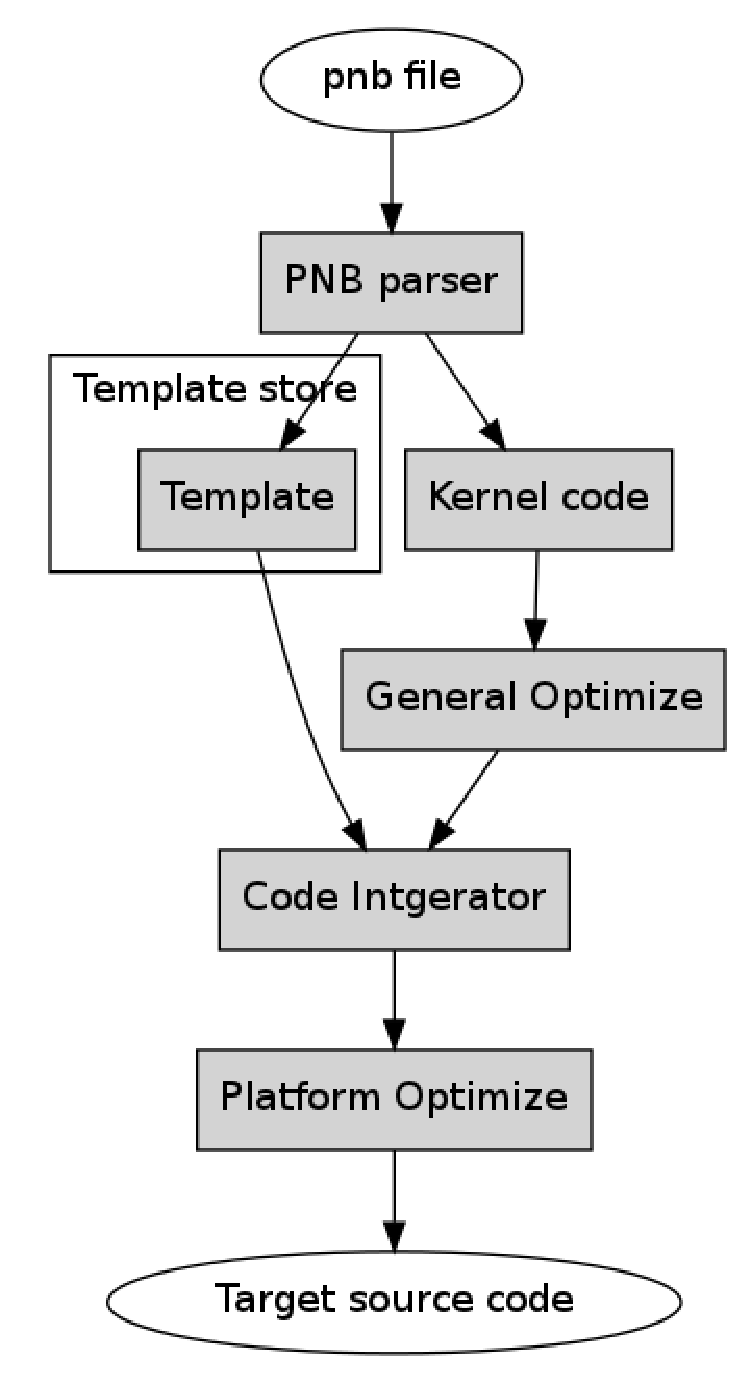
\includegraphics[width=2.0in]{block.eps}
\caption{Block diagram showing the implementation of PNBsolver}
\label{fig_block}
\end{figure}

\subsection{PNBSolver Parser}

The simplified EBNF grammar for the PNBsolver language is shown in Figure \ref{fig_grmr}. 
As shown in the figure, the file allows one or more kernels, but code is generated for only one kernel.
This is designed to support future extensions, where the output of a kernel can be passed to the input of another kernel. After parsing, the expression statement is captured in two
expression objects, the inner expression object and the outer expression object. All expressions in a ``pnb'' file are made of variables defined in the declaration section. To use a constant
inside the expression statement, it should be declared as a constant and use the variable name in the expression statement. As a rule, the read statements should be defined before
the expression statement, and write statements after the expression statement. This seems logical as a program usually requires reading before the calculation and writing after the
 calculation. The EBNF rules for \texttt{variabledeclaration}, \texttt{writestmts}, and \texttt{parameters} are not shown in the figure to provide clarity. 
 
\begin{figure}[!t]
\centering
\begin{lstlisting}[style=AMMA, language=PNB]

grammar PNBsolver;

content
	: kernels  execute "." EOF 
	;

kernels
	: ("kernel"  ID "in" ID declarations readstmts 
            expressionstmt writestmts "endkernel")+
	;

declarations
	: (type variabledeclaration)+
	;

execute 
	: "generate" platform ("[" parameters "]")? mode ID
	;

platform
	: "CUDA"|"OMP"|"MPI"|"OCL"
	;

mode
	: "ACCURATE"|"AVERAGE"|"FAST"
	; 
type
	: "vector"|"scalar"|"constant"
	;  
            
expressionstmt
	: IDENTIFIER "=" (expression)? "SUM" expression 
	;

expression
	: multidiv( "+" multidiv|   "-" multidiv )* 
	;

multidiv
	: atom ("*" atom |"/" atom)* 
	; 

atom
	: IDENTIFIER
	| "(" expression ")"
	| "exp" expression 
	| "pow" "("expression "," NUMBER ")" 
	;
           
readstmts
	: ("read" STRING "," STRING)*
	;
\end{lstlisting}
\caption{Simplified EBNF grammar of PNBsolver}
\label{fig_grmr}
\end{figure}

\subsection{PNBsolver code generator}
The PNBsolver parser can identify the inputs and outputs for the kernel. The code generator inserts declarations and initialization (if any) into the program. The core computation
code is generated as shown in Figures \ref{fig_first_case} and \ref{fig_second_case}. These two code sections are inserted into the template identified by mode and 
platform. To add a new algorithm, we have
defined a new template and configured the parser to route through a different code generator. The same approach can be used to support a language other than C. In Section \ref{sec_cmp},
we generate FORTRAN code using a FORTRAN code generator. There are four ``C'' templates available in the template store and are  explained in the following subsections. 

\subsubsection{Parallel CPU (OpenMP and MPI) tree code templates}
The tree code used for PNBsolver is adapted from \cite{krasny1}. We developed parallel versions of the tree code in MPI and OpenMP. More details about the speedup, 
error and execution time are included in Section \ref{sec_more}. To complete a CPU tree code template, we need: 1) Taylor coefficients, 2) Direct 
implementation, and 3) Tree code parameters such as  MAXPARNODE, ORDER (taylor coefficient order) and THETA (MAC). PNBsolver sets default values for all of these 
parameters, but this can be customized by the user as shown later in Figure \ref{fig_yukawa}. 

\begin{figure}[!t]
\centering
\begin{lstlisting}[style=AMMA, language=C]
struct tnode {
    int numbodies,begin,end;
    double x_min, y_min, z_min,x_max, y_max,z_max;
    double x_mid,y_mid,z_mid,radius;
    int level,children,exist_ms;
    double ***moments;
    struct tnode* child[8];
};
\end{lstlisting}
\caption{Structure \texttt{tnode} in the template}
\label{fig_tnode}
\end{figure}

\textit{Providing Taylor coefficients: }
The parameter value TAYLOR is used to find the Taylor coefficients. The PNBsolver code generator reads the file specified as the parameter value of TAYLOR
and looks for a function with signature \texttt{comptcoeff (struct tnode *t)}, where \texttt{tnode} is a structure representing the tree node. In this function, the position of 
an interacting body can also be  accessed. The declaration of structure \texttt{tnode} is shown in Figure \ref{fig_tnode}. The values of the Taylor coefficients
should be set in a 3D array of size ORDER. In addition to the \texttt{comptcoeff} function, users can add two more functions: \texttt{setup()} and \texttt{teardown()}, for declaring 
values that might be required for the computation. These two functions are executed only once before and after the tree creation, while the \texttt{comptcoeff} function is executed
for every target that satisfies THETA. All of these functions  can access the user-specified parameters and some global parameters which include NUMPARS (number of bodies).
If PNBsolver is executed with a TAYLOR parameter, it will look for a file specified as the value. If PNBsolver cannot find the file in the current directory,
a file having the above three function signatures will be created. PNBsolver uses Taylor coefficients mentioned in  \cite{krasny1} 
if TAYLOR is not specified  and it is found effective for Force and Potential calculations. 

\begin{figure}[!t]
\centering
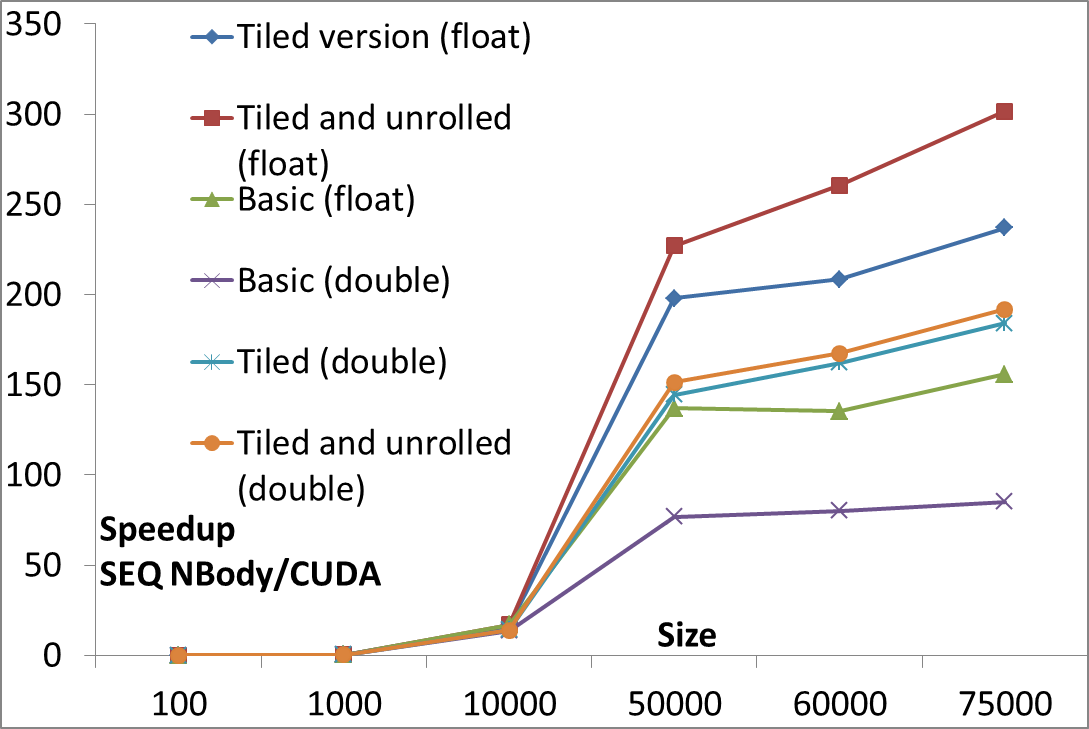
\includegraphics[width=4.0in]{cuda_plot3.eps}
\caption{Effect of optimization techniques (Tiling and unrolling) for Coulomb potential}
\label{fig_cuda3}
\end{figure}

\subsubsection{Parallel GPU template for direct computation}
For the GPU implementation using the direct summation, we have used two optimization techniques: 1) Tiling (partitioning of the computation domain into smaller tiles) 
 with shared memory, and 2) Loop unrolling (replacing a loop with similar independent statements). The effect of these  optimizations for Coulomb Potential is shown in Figure \ref{fig_cuda3}. In the figure,  the direct version 
is the case when the kernel code generated 
 was executed as a CUDA kernel without any modifications on a Tesla M2070. All kernels in the GPU template can be executed for \texttt{double} and 
\texttt{float} mode. In the figure,  Speedup is defined as the ratio of execution time of sequential implementation of Coulomb potential on a CPU to that of the CUDA implementation.
 Every reading is an average value of at least three of the same executions.    

\subsubsection{Parallel GPU tree code template}
The implementation we use for GPU tree code is adapted from \cite{gputree}. Our current implementation only supports zeroth ORDER; hence, there is no need to specify Taylor
coefficients for tree code implementation. 


\subsection{Modes of operation}
There are three modes of operation for PNBsolver: 1) ACCURATE, 2) AVERAGE, and 3) FAST. The execution time of the problem decreases from ACCURATE to FAST and error decreases
from FAST to ACCURATE. This is achieved by varying the parameters ORDER and THETA. The effect of these two parameters for two problems executed for a PNBsolver OpenMP solution
for a fixed size is shown in Figures \ref{fig_order} and \ref{fig_theta}. As seen from the figure, as the ORDER increases, error is less but the program takes longer to finish execution.  
In the case of THETA, the program finishes faster for higher values of THETA, but has increased errors due to lowered threshold for using particle-cluster interaction. 
Unless specified, the THETA value is set to 0.5 as a default. 

\begin{figure}[!t]
\centering
\includegraphics[width=3.5in]{order.eps}
\caption{Effect of ORDER in error and time}
\label{fig_order}
\end{figure}

\begin{figure}[!t]
\centering
\includegraphics[width=3.5in]{theta.eps}
\caption{Effect of THETA in error and time}
\label{fig_theta}
\end{figure}

 
\begin{table}[!t]
\caption{Three modes of operation and corresponding tuning parameters }
\label{tbl_pars}
\centering

\begin{tabular}{|l|l|l|l|} \hline
Platform & Mode & Algorithm &Parameters\\\hline
\multirow{3}{*}{GPU (CUDA)} & ACCURATE & DIRECT& DOUBLE \\
& AVERAGE & DIRECT & FLOAT \\
& FAST & TREE & \\ \hline
\multirow{3}{*}{CPU (OpenMP \& MPI)} & ACCURATE &TREE& ORDER=6 \\
& AVERAGE&TREE & ORDER=4 \\
& FAST &TREE& ORDER=1 \\\hline
\end{tabular}
\end{table}

PNBsolver uses these tuning parameters to allow programmers to control the error and execution of generated programs. The parameter values set through a mode can be 
overridden by specifying the parameter in the \texttt{generate} clause. The value of relevant parameters for the three modes are shown in Table \ref{tbl_pars}. 
As shown in the table, GPU implementations (currently only supported in CUDA) in the ACCURATE mode gives the most accurate results using direct computation with \texttt{double}  precision for all computation variables, the AVERAGE mode also uses direct computation, but with \texttt{float} precision for all variables. Hence, the AVERAGE mode gives faster execution time than ACCURATE mode, but less accurate results. In the FAST mode, CUDA implementations make use of the Tree code algorithm to give the fastest execution time, but even less accurate results compared to the AVERAGE mode. In CPU implementations (MPI and OpenMP), the Tree code algorithm is used in all three cases, such that the speed and accuracy are controlled by tuning the ORDER variable. When order is set at a higher value, the algorithm provides accurate results, but execution time is longer, as shown in Figure \ref{fig_order}.   

\section{PNBsolver and handwritten code comparison}
\label{sec_cmp}

In this section, we compare the execution time of two kernels generated by PNBsolver with that of handwritten code from expert programmers.  

\subsection {Yukawa potential (screened Coulomb potential) calculation}

The electrostatic Yukawa energy potential at the $i$th charge $Y_i$, due to the N mutually interacting  charged particles 
 with coordinates $R$  and partial charges $Q_i(i=1,N)$, is calculated as shown in Equation \ref{eqn_yukawa}.

\begin{equation}
\label{eqn_yukawa}
Y_i=Q_i \sum \limits_{j=1,j!=i}^{N} \frac{Q_je^{-|R_i-R_j|}}{|R_i- R_j|} 
\end{equation}

The PNBsolver representation for Yukawa interactions is shown in Figure \ref{fig_yukawa}. The code is generated for an MPI version with parameters: 
TAYLOR and MAXPARNODE (line 20). Since the code is generated for AVERAGE mode, from Table \ref{tbl_pars}, ORDER=4 and default value of THETA is 0.5.   
It is assumed that the Taylor coefficient implementation is available in a file ``comptt.c'' 

\begin{figure}[!t]
\centering
\begin{lstlisting}[style=AMMA, language=PNB]
kernel Yukawa in R

// Kernel declarations
	scalar Y
	scalar Q
	constant KAPPA=1.0
	
	read "R_1,R_2,R_3,Q", "data.dat"

	//Actual computation
	Y=Q SUM(Q*exp(-KAPPA*R)/R)

	// Write Yukawa potential to file 
	write "Y", "out.dat"
	
endkernel

generate MPI AVERAGE Yukawa 
//Parameters
	[TAYLOR=comptt.c, MAXPARNODE=100]. 
\end{lstlisting}
\caption{Screened (Yukawa) potential kernel in space R using PNBsolver}
\label{fig_yukawa}
\end{figure}

\textit{Comparison: }
We compared the execution time of MPI code generated by PNBsolver to to Li et al. \cite{li}.  To make the comparison as accurate as possible, 1) we set the same parameter 
values for the version in test, 2) used a FORTRAN template instead of the C template, and 3) MPI code generated by PNBsolver is executed with one process. 
The execution times were recorded for the size varying from 1000 (1k) to 500k. The execution times are shown in Figure \ref{fig_cmp}, where FORTRAN screened \cite{li} is the
version in test (FORTRAN Screened (Li) in figure) and FORTRAN screened (PNBsolver) is the generated version. As seen in Figure \ref{fig_cmp}, generated code executed nearly as fast as the sequential hand written code. 
 

\begin{figure}[!t]
\centering
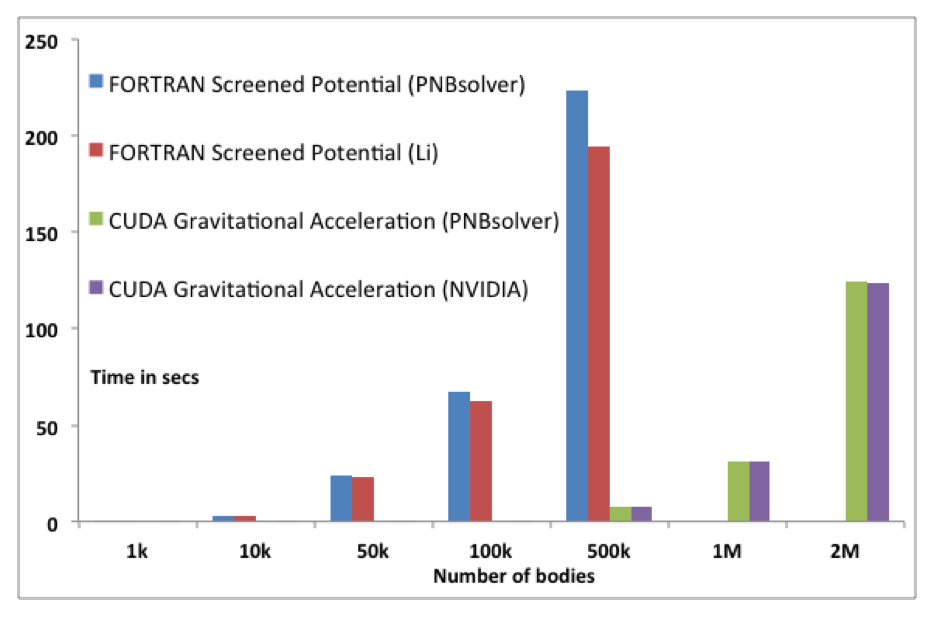
\includegraphics[width=3.5in]{cmp.eps}
\caption{Execution time comparison of hand-written code with generated code}
\label{fig_cmp}
\end{figure}

\subsection{Gravitational acceleration}
The equation to calculate gravitational acceleration is similar to Equation \ref{eqn_force} without the $M_i$ in the outer loop. The PNBsolver code  for Force is 
shown in Figure \ref{fig_force}. We compared the PNBsolver acceleration with an acceleration implementation from the NVIDIA CUDA installation 
package\footnote{CUDA SDK, \url{http://developer.nvidia.com/cuda-cc-sdk-code-samples}}. We slightly modified the NVIDIA code to make more precise comparisons. For all
GPU plots, the execution time includes: 1) Time to allocate memory in GPU, 2) Time to transfer memory from CPU to GPU, 3) GPU execution, and 4) Copying results back
to CPU. We  added code to pass the input values to the GPU before execution and also code to read back after execution. However, we used the 
\texttt{nbody\_kernel.cu} file, which performs  the actual implementation for comparison. 

\textit{Comparison: }
We compared the execution time of the NVIDIA implementation of gravitational acceleration with the generated code of PNBsolver. The number of bodies were varied from 1k to
2M. For PNBsolver, the CUDA direct summation was used with single point precision. The execution times of both of these versions are shown in Figure \ref{fig_cmp}. 
As seen from the figure, PNBsolver can generate code that is as fast as the CUDA implementation. 












\section{More N-body problems}
\label{sec_more}

In this section, we explain the speedup and the errors (numerical deviation from the expected results) of a few N-body problems in three different architectures: 1) Shared memory (OpenMP), 
2) Distributed memory (MPI),  and 3) GPU (CUDA). The analysis of OpenMP and MPI programs is given in the following subsection and CUDA programs is provided in 
subsection \ref{sec_cuda}.

\subsection{Analysis of OpenMP and MPI programs}
For the OpenMP and MPI program analysis, in addition to the Force (Equation \ref{eqn_force}) and  Yukawa potential (Equation \ref{eqn_yukawa}), we generated code for the 
Coulomb potential which is calculated as shown in Equation \ref{eqn_coul}. The PNBsolver representation of the Coulomb potential is shown in Figure \ref{fig_coul}. 

\begin{equation}
\label{eqn_coul}
V_i=Q_i \sum \limits_{j=1, j \ne i}^{N} \frac{Q_j}{|R_i- R_j|} 
\end{equation}

\begin{figure}[!t]
\centering
\begin{lstlisting}[style=AMMA, language=PNB]
kernel Potential in R

	scalar Y, Q
	
	read "R_1,R_2,R_3,Q", "data.dat"

	//Actual computation
	V=Q SUM(Q/R)

	// Write Yukawa potential to file 
	write "V", "out.dat"
	
endkernel

generate OMP AVERAGE Potential. 
\end{lstlisting}
\caption{Coulomb potential kernel in space R using PNBsolver}
\label{fig_coul}
\end{figure}

\subsubsection{Execution environment}
The MPI and OpenMP programs were executed in a cluster with eight nodes. The programs read positions and charges from a file of 5 million records. We modified the generated
code to include a direct implementation on every program to verify the accuracy of the implementation. The programs were executed for a number of bodies ranging from 5k to 500k.
  
\subsubsection{Speed up of MPI and OpenMP programs}
To evaluate our parallel implementations of the tree code algorithms in  OpenMP and MPI platforms, the speedup (ratio of the sequential tree code execution time to that of the
parallel tree code), as shown in Figure \ref{fig_ompmpi1}, is plotted against the number of threads for OpenMP and processes for MPI programs. As shown in the graph, 
our parallel implementation gave a linear speedup until eight (number of nodes in the cluster) threads/processes. For more computation intensive equations, 
executing with more threads or processes than the available resources can slow down the program to a considerable rate as in the case of 
Screened Coulomb potential in Figure \ref{fig_ompmpi1}. 
In Figure \ref{fig_ompmpi2}, the speedup is plotted against 
the number of bodies, where relative speedup is defined as the ratio of execution time of a sequential program to that of the tree code program. 
In this case, super linear speedup is observed with the tree code algorithm. 

\begin{figure}[!t]
\centering
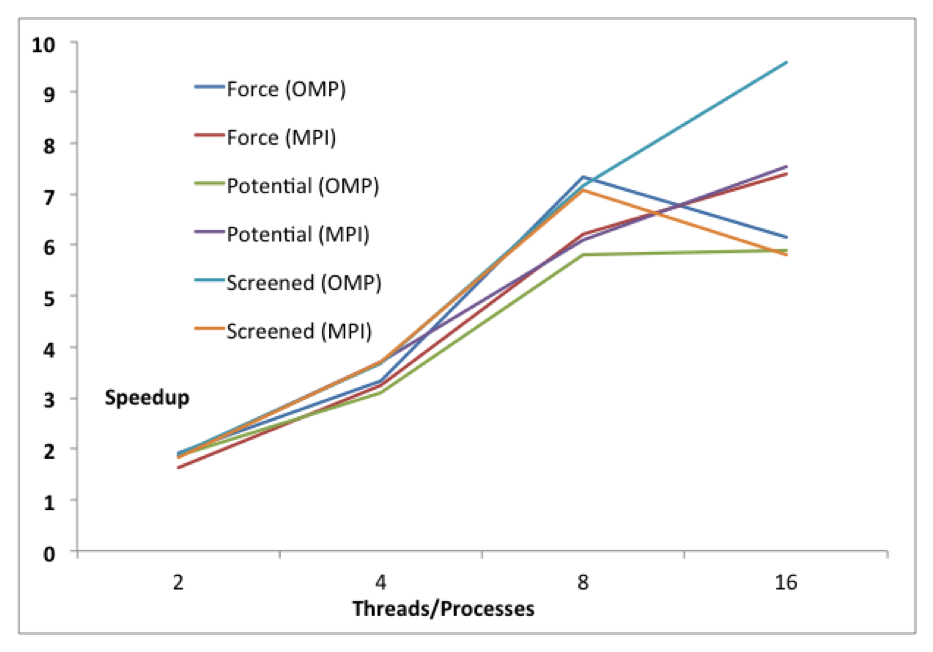
\includegraphics[width=4.0in]{ompmpi1.eps}
\caption{Speedup of tree code programs with sequential tree code}
\label{fig_ompmpi1}
\end{figure}

\begin{figure}[!t]
\centering
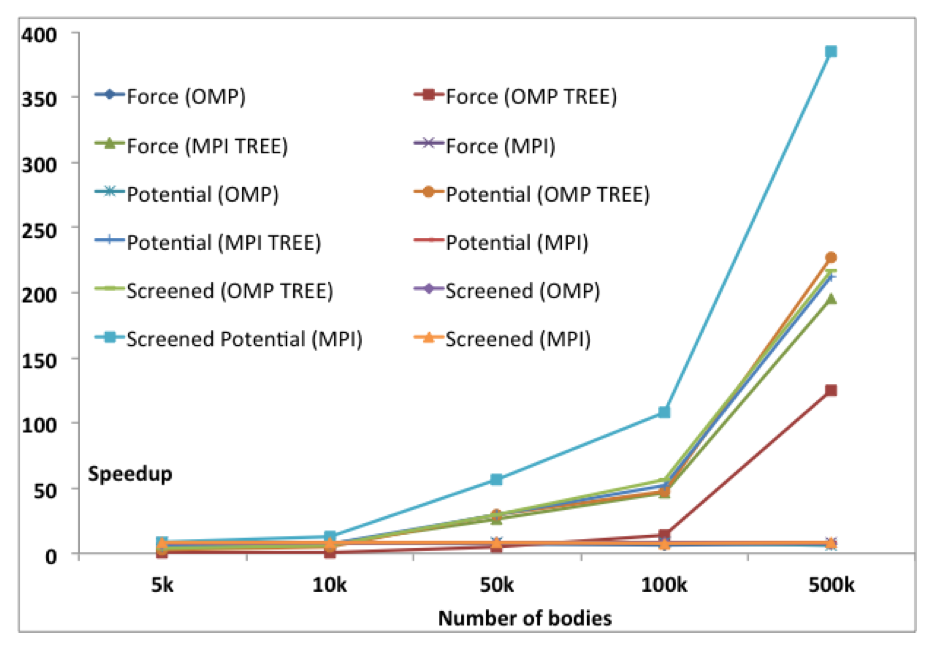
\includegraphics[width=4.0in]{ompmpi2.eps}
\caption{Speedup of tree code programs with sequential direct code}
\label{fig_ompmpi2}
\end{figure}

\subsection{Analysis of CUDA programs}
\label{sec_cuda}

For CUDA analysis, we included the expression  shown in Equation  \ref{eqn_vortex} \cite{vortex} for computing vortex sheet motion in 3D flow. The PNBsolver file
is shown in Figure \ref{fig_vortex}. 

\begin{equation}
\label{eqn_vortex}
v_i= -\sum \limits_{j=1, j\ne i}^{N} \frac{W_j}{{({|R_i- R_j|}^2+{\delta}^2})^3} 
\end{equation}
\begin{figure}[!t]
\centering
\begin{lstlisting}[style=AMMA, language=PNB]
kernel Vortex in R

	scalar W
	vector V
	constant DELATSQ=0.00125	

	read "R_1,R_2,R_3,W", "data.dat"

	V= SUM(W/((R_*R_+DELTASQ)(R_*R_+DELTASQ) (R_*R_+DELTASQ))

	write "V_1,V_2,V_3", "out.dat"
	
endkernel
generate CUDA AVERAGE Vortex. 
\end{lstlisting}
\caption{Coulomb potential kernel in space R using PNBsolver}
\label{fig_vortex}
\end{figure}

\subsubsection{Execution environment}
We executed the generated code on a Tesla M2070 GPU card. The generated code was modified to verify the results for accuracy with the direct implementation. Similar
to the OpenMP and MPI implementations, the generated code read from a file of five million records and programs were executed from a number of bodies ranging from 10K to
5M values. 


\subsubsection{Speedup of CUDA programs}
The OpenMP direct implementation of the Coulomb potential for five million bodies executed with eight threads took almost two days to finish execution, while the CUDA FAST
version finished in less than a few seconds. For plotting, we defined relative speedup as the ratio of execution time of CUDA direct double or float to that of CUDA tree code. The speedups
for the four equations are shown in Figure \ref{fig_cuda1} and relative errors recorded in the computation are shown in Figure \ref{fig_cuda2}. A relative error is defined
as the ratio of the highest absolute error to the highest value in direct summation. As shown in Figures \ref{fig_cuda1} and \ref{fig_cuda2}, PNBsolver can generate 
CUDA programs that are fast and more accurate. From Figure \ref{fig_cuda1}, it can be seen that the speedup of float is less than
double. This is because the execution time of float is less compared to double. Therefore  the speedup with the tree code is less. 

\begin{figure}[!t]
\centering
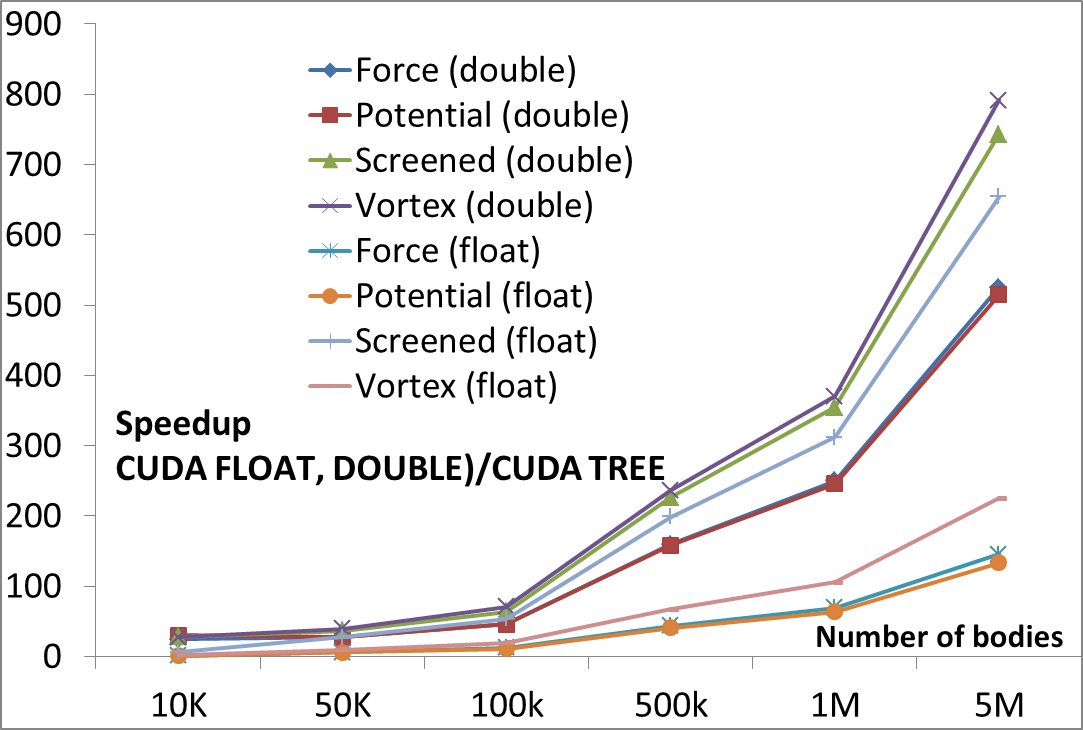
\includegraphics[width=3.5in]{cuda_plot1.eps}
\caption{Speedup of CUDA tree code with direct CUDA}
\label{fig_cuda1}
\end{figure}

\begin{figure}[!t]
\centering
\includegraphics[width=3.5in]{cuda_plot2.eps}
\caption{Error in  CUDA tree code programs}
\label{fig_cuda2}
\end{figure}

\section{Related works}
\label{related}

We have classified the related works into three categories, as explained in the following subsections. 

\subsection{N-body solutions}

A  major advance in N-body simulation  was the introduction of the GRAPE (Gravity PiPE) series of special-purpose computers \cite{grape}.
But recent works show that comparable speedup can be achieved through GPUs \cite{grapegpu}. 
AMBER \cite{pearlman} is a package  of computer programs written in FORTRAN to simulate  the structural  and energetic
properties  of molecules. AMBER used a non-bonded cutoff sphere for applying approximation in  N-body energy equations. AMBER 4.0 
adds parallelism to modules of the program. NAMD \cite{kale} is a parallel simulation program written in C++ and used 
to simulate the behavior of bio-molecular systems. NAMD2 uses Converse (a portable runtime framework) to support interoperability 
between different parallel paradigms. FMM-Yukawa \cite{ jhuang} is a FORTRAN program package for fast evaluation of the screened 
Coulomb interaction of N particles. Programs can execute in linear time for nearly uniform particle distributions. Compared to 
PNBsolver, these programs have targeted a specific field and to a specific N-body problem.

MATLAB\footnote{MATLAB, \url{http://www.mathworks.com}} is a high performance language for technical computing where solutions and problems are
expressed in mathematical notations. Being a general tool, it is highly improbable to have the expressiveness or performance as compared
to the domain-specific PNBsolver, which can be extended to support more algorithms by adding templates and allow programmers to fine-tune
these algorithms based on their specific problem. 
%Popular parallel paradigms such as  MapReduce  are available in cloud environments

\subsection{Tree code algorithms}
Cheng et. al. \cite{cheng} used an adaptive quad tree structure to develop an adaptive fast solver for a modified Helmholtz equation in
two dimensions. Ossmani et. al. \cite{ossmani} used a tree based data structure to evaluate efficiency of a multi-scale hybrid 
grid-particle vortex method. Krasny et. al.  \cite{krasny1} used a tree code algorithm to compute non-bonded particle-cluster and 
cluster-cluster interaction. They also used an oct-tree data structure and implemented different tree traversing techniques specific to different 
boundary conditions. Krasny et. al. \cite{krasny2} implemented the tree code in Cartesian coordinates and used a recurrence relation 
to compute the Taylor coefficient for evaluating sums of multi-quadric radial basis function (RBF). Xu et. al. \cite{xu} used a tree code 
algorithm for calculating polarized Coulomb interaction of an N-body system. Li et. al. \cite{li} used the algorithm
for evaluating electrostatic potential of screened Coulomb interaction using a new recurrence relation. 
Baczewski et. al. \cite{baczewski} presented an Accelerated Cartesian Expansion (ACE) method to evaluate periodic 
Helmholtz, Coulomb and Yukawa potential using $\mathcal{O}(N)$ operations and $\mathcal{O}(N)$ storage using different approximations in
both tree building and tree traversing.  \cite{hybridtree2015} showed a hybrid tree algorithm for reducing calculation and communication cost of 
collision-less N-body simulations.
All of these works represent different variations of the original tree code algorithm.
Because PNBsolver is more focused on the approach than to a specific algorithm, PNBsolver can support any of these. 

\subsection{Modeling in parallel programming}
There have been several modeling efforts in solving HPC applications \cite{rithu1,rithu2}. Liszt \cite{liszt} is a DSL for constructing mesh-based solvers that 
can generate MPI, pthreads, and CUDA code. Similarly, SPIRAL \cite{spiral} generates high performance code of Digital Signal Processing (DSP) transforms. 
Popular parallel paradigms such as MapReduce are available in cloud environments through similar approaches \cite{mapredoop}.
CODE \cite{code} and GASPARD \cite{gaspard} are two graphical programming environments unlike PNBsolver, which is a modeling tool. 
PPModel \cite{sc11,acmse} is a graphical modeling tool that helps programmers to identify parallel sections in a program and re-target to a different 
platform.  PPModel is a general tool and hence can only transform the code to the target platform without any optimizations.
IPT \cite{ipt} can be used to semi-automatically generate parallel programs executable in MPI, OpenMP, and CUDA platforms and help the HPC domain experts to learn about 
these parallel platforms through observation and comparison.

\section{Future work and Conclusion}
\label{conclusion}

PNBsolver has been implemented to show that our two-stage modeling approach can be applied to parallel programs. In the implementation, tree code algorithms are generated
for the specified order for MPI/OpenMP programs, and zero order for CUDA programs. Extending a GPU program also for the specified order is a future direction of work.
Another possible direction would be adding more templates for supporting other platforms and paradigms like OpenCL.   


N-body problems involve computing interactions of multiple bodies in a 3D space. The existing solutions work on a specific problem, specific algorithm, and specific platform. 
In this paper, we introduce a domain-specific language called PNBsolver, which can express the computations in an N-body problem in a manner that is oblivious to their implementation, 
platform, and algorithmic details without compromising the execution time. PNBsolver can be executed in three modes: 1) FAST, 2) AVERAGE, and 3) ACCURATE modes in three popular 
parallel programming paradigms (CUDA, OpenMP and MPI). Modes are defined based on the target platform (e.g., ACCURATE mode on a GPU uses a double precision algorithm in CUDA, 
and the ACCURATE mode on a CPU uses a 10-order tree code algorithm). The speedup and errors were analyzed for four commonly seen N-body interactions. We compared
the execution time of the generated code with that of handwritten code by expert programmers to show that the execution time is not compromised. PNBsolver was successfully 
applied to five N-body problems and their corresponding speedups and errors were plotted.




% conference papers do not normally have an appendix


% use section* for acknowledgement
\section*{Acknowledgment}
This work was made possible in part by a grant of high performance computing resources and technical support from the Alabama Supercomputer Authority.




% trigger a \newpage just before the given reference
% number - used to balance the columns on the last page
% adjust value as needed - may need to be readjusted if
% the document is modified later
%\IEEEtriggeratref{8}
% The "triggered" command can be changed if desired:
%\IEEEtriggercmd{\enlargethispage{-5in}}

% references section

% can use a bibliography generated by BibTeX as a .bbl file
% BibTeX documentation can be easily obtained at:
% http://www.ctan.org/tex-archive/biblio/bibtex/contrib/doc/
% The IEEEtran BibTeX style support page is at:
% http://www.michaelshell.org/tex/ieeetran/bibtex/
\bibliographystyle{IEEEtran}
%\bibliography{init_draft}

% Generated by IEEEtran.bst, version: 1.13 (2008/09/30)
\begin{thebibliography}{10}
\providecommand{\url}[1]{#1}
\csname url@samestyle\endcsname
\providecommand{\newblock}{\relax}
\providecommand{\bibinfo}[2]{#2}
\providecommand{\BIBentrySTDinterwordspacing}{\spaceskip=0pt\relax}
\providecommand{\BIBentryALTinterwordstretchfactor}{4}
\providecommand{\BIBentryALTinterwordspacing}{\spaceskip=\fontdimen2\font plus
\BIBentryALTinterwordstretchfactor\fontdimen3\font minus
  \fontdimen4\font\relax}
\providecommand{\BIBforeignlanguage}[2]{{%
\expandafter\ifx\csname l@#1\endcsname\relax
\typeout{** WARNING: IEEEtran.bst: No hyphenation pattern has been}%
\typeout{** loaded for the language `#1'. Using the pattern for}%
\typeout{** the default language instead.}%
\else
\language=\csname l@#1\endcsname
\fi
#2}}
\providecommand{\BIBdecl}{\relax}
\BIBdecl

\bibitem{babage}
L.~F. Menabrea, ``Sketch of the analytic engine invented by charles babbage,''
  \emph{Biblioth{\'e}que Universelle de Gen{\'e}ve}, no.~82, September 1842.

\bibitem{gpgpu}
J.~D. Owens, D.~Luebke, N.~Govindaraju, M.~Harris, J.~Kr{\"u}ger, A.~Lefohn,
  and T.~J. Purcell, ``A survey of general-purpose computation on graphics
  hardware,'' \emph{Computer Graphics Forum}, vol.~26, no.~1, pp. 80--113,
  2007.

\bibitem{comparison}
A.~R. Brodtkorb and T.~R. Hagen, ``A comparison of three commodity-level
  parallel architectures: Multi-core cpu, cell be and gpu,'' in
  \emph{Proceedings of the International Conference on Mathematical Methods for
  Curves and Surfaces}, T{\o}nsberg, Norway, July 2008, pp. 70--80.

\bibitem{openmp}
R.~Chandra, L.~Dagum, D.~Kohr, D.~Maydan, J.~McDonald, and R.~Menon,
  \emph{Parallel programming in {O}pen{MP}}.\hskip 1em plus 0.5em minus
  0.4em\relax Morgan Kaufmann Publishers Inc., 2001.

\bibitem{liszt}
Z.~DeVito, N.~Joubert, F.~Palacios, S.~Oakley, M.~Medina, M.~Barrientos,
  E.~Elsen, F.~Ham, A.~Aiken, K.~Duraisamy, E.~Darve, J.~Alonso, and
  P.~Hanrahan, ``Liszt: a domain specific language for building portable
  mesh-based pde solvers,'' in \emph{Proceedings of the International
  Conference for High Performance Computing, Networking, Storage and Analysis},
  Seattle, Washington, 2011, pp. 9:1--9:12.

\bibitem{trilinos}
M.~A. Heroux, R.~A. Bartlett, V.~E. Howle, R.~J. Hoekstra, J.~J. Hu, T.~G.
  Kolda, R.~B. Lehoucq, K.~R. Long, R.~P. Pawlowski, E.~T. Phipps, A.~G.
  Salinger, H.~K. Thornquist, R.~S. Tuminaro, J.~M. Willenbring, A.~Williams,
  and K.~S. Stanley, ``An overview of the trilinos project,'' \emph{ACM
  Transactions on Mathematical Software}, vol.~31, no.~3, pp. 397--423, 2005.

\bibitem{spiral}
M.~P{\"u}schel, J.~M.~F. Moura, J.~Johnson, D.~Padua, M.~Veloso, B.~W. Singer,
  J.~Xiong, F.~Franchetti, A.~Ga\v{c}i\'{c}, Y.~Voronenko, K.~Chen, R.~W.
  Johnson, and N.~Rizzolo, ``{SPIRAL}: Code generation for {DSP} transforms,''
  \emph{Proceedings of the IEEE, special issue on Program Generation,
  Optimization, and Adaptation}, vol.~93, no.~2, pp. 232--275, 2005.

\bibitem{modeldriven}
D.~Schmidt, ``Model-driven engineering,'' \emph{IEEE Computer}, vol.~39, no.~2,
  pp. 25--32, 2006.

\bibitem{ds1}
A.~L\'{e}deczi, A.~Bakay, M.~Mar\'{o}ti, P.~V\"{o}lgyesi, G.~Nordstrom,
  J.~Sprinkle, and G.~Karsai, ``Composing domain-specific design
  environments,'' \emph{IEEE Computer}, vol.~34, no.~11, pp. 44--51, 2001.

\bibitem{dsml}
J.~Sprinkle, M.~Mernik, J.-P. Tolvanen, and D.~Spinellis, ``{Guest Editors'
  Introduction}: {W}hat kinds of nails need a {D}omain-{S}pecific hammer?''
  \emph{IEEE Software}, vol.~26, no.~4, pp. 15--18, 2009.

\bibitem{modeldriven1}
C.~Atkinson and T.~Kuhne, ``Model-driven development: {A} metamodeling
  foundation,'' \emph{IEEE Software}, vol.~20, no.~5, pp. 36--41, 2003.

\bibitem{dsl}
M.~Mernik, J.~Heering, and A.~M. Sloane, ``When and how to develop
  domain-specific languages,'' \emph{ACM Computing Surveys}, vol.~37, no.~4,
  pp. 316--344, 2005.

\bibitem{diacu}
F.~Diacu, ``The solution of the n-body problem,'' \emph{The Mathematical
  Intelligencer}, vol.~18, no.~3, pp. 66--70, Nov 1996.

\bibitem{watson}
K.~M. Watson, ``Multiple scattering and the many-body problem - applications to
  photomeson production in complex nuclei,'' \emph{Phys. Rev.}, vol.~89, no.~3,
  pp. 575--587, Feb 1953.

\bibitem{jastrow}
R.~Jastrow, ``Many-body problem with strong forces,'' \emph{Phys. Rev.},
  vol.~98, no.~5, pp. 1479--1484, Jun 1955.

\bibitem{sasai}
M.~Sasai and P.~G. Wolynes, ``Stochastic gene expression as a many-body
  problem,'' \emph{Proceedings of the National Academy of Science, PNAS}, vol.
  100, no.~5, pp. 2374--2379, Mar 2003.

\bibitem{carlson}
J.~Carlson, J.~Kogut, and V.~R. Pandharipande, ``Quark model for baryons based
  on quantum chromodynamics,'' \emph{Phys. Rev. D}, vol.~27, no.~1, pp.
  233--243, Jan 1983.

\bibitem{barnes}
J.~Barnes and P.~Hut, ``A hierarchical o(n log n) force-calculation
  algorithm,'' \emph{Nature}, vol. 324, pp. 446--449, Dec 1986.

\bibitem{krasny1}
R.~Krasny and Z.-H. Duan, ``Treecode algorithms for computing nonbonded
  particle interactions,'' in \emph{Computational Methods for Macromolecules:
  Challenges and Applications}, T.~Schlick and H.~H. Gan, Eds.\hskip 1em plus
  0.5em minus 0.4em\relax Springer Berlin Heidelberg, 2002, pp. 359--380.

\bibitem{krasny2}
R.~Krasny and L.~Wang, ``Fast evaluation of multiquadric rbf sums by a
  cartesian treecode,'' \emph{SIAM Journal on Scientific Computing}, vol.~33,
  no.~5, pp. 2341--2355, Sep 2011.

\bibitem{xu}
Z.~Xu, ``Treecode algorithm for pairwise electrostatic interactions with
  solvent-solute polarization,'' \emph{Phys. Rev. E}, vol.~81, no.~2, p.
  020902, Feb 2010.

\bibitem{mac}
J.~K. Salmon and M.~S. Warren, ``{Skeletons from the Treecode Closet},''
  \emph{Journal of Computational Physics}, vol. 111, pp. 136--155, 1994.

\bibitem{li}
P.~Li, H.~Johnston, and R.~Krasny, ``A cartesian treecode for screened coulomb
  interactions,'' \emph{Journal of Computational Physics}, vol. 228, no.~10,
  pp. 3858 -- 3868, Jun 2009.

\bibitem{vortex}
K.~Lindsay and R.~Krasny, ``A particle method and adaptive treecode for vortex
  sheet motion in three-dimensional flow,'' \emph{Journal of Computational
  Physics}, vol. 172, no.~2, pp. 879--907, September 2001.

\bibitem{code1}
``Johnston tree code,'' \url{http://www.math.umass.edu/~johnston/}, [Online;
  accessed 01-March-2015].

\bibitem{code2}
``Barnes tree code,''
  \url{http://www.ifa.hawaii.edu/~barnes/treecode/treeguide.html}, [Online;
  accessed 01-March-2015].

\bibitem{code3}
``Elucidation tree code,'' \url{https://github.com/Elucidation/Nbody_cpp},
  [Online; accessed 01-March-2015].

\bibitem{ewald}
D.~Liu, Z.-H. Duan, R.~Krasny, and J.~Zhu, ``Parallel implementation of the
  treecode ewald method,'' in \emph{Proceedings of the International Parallel
  and Distributed Processing Symposium}, Santa Fe, NM, April 2004.

\bibitem{gputree}
K.~P. Martin~Burtscher, ``An efficient cuda implementation of the tree-based
  barnes hut n-body algorithm,'' in \emph{Chapter 6 in GPU Computing Gems
  Emerald Edition}, W.~mei W.~Hwu, Ed.\hskip 1em plus 0.5em minus 0.4em\relax
  Elsevier Inc., 2011, pp. 75--92.

\bibitem{bonzai}
J.~B{\'e}dorf, E.~Gaburov, and S.~P. Zwart, ``Bonsai: A {GPU} {T}ree-{C}ode,''
  2012.

\bibitem{grape}
J.~Makino and M.~Taiji, \emph{Scientific {S}imulations with {S}pecial-{P}urpose
  {C}omputers - the {GRAPE} {S}ystems}, 1st~ed.\hskip 1em plus 0.5em minus
  0.4em\relax New York, NY: John Wiley, 1998.

\bibitem{grapegpu}
R.~G. Belleman, J.~B\'{e}dorf, and S.~F. Portegies~Zwart, ``{High performance
  direct gravitational N-body simulations on graphics processing units II: An
  implementation in CUDA},'' \emph{New Astronomy}, vol.~13, no.~2, pp.
  103--112, 2008.

\bibitem{pearlman}
D.~A. Pearlman, J.~W. Case, David A.~Caldwell, W.~S. Ross, T.~E. Cheatham,
  S.~DeBolt, D.~Ferguson, G.~Seibel, and P.~Kollman, ``{AMBER}, a package of
  computer programs for applying molecular mechanics, normal mode analysis,
  molecular dynamics and free energy calculations to simulate the structural
  and energetic properties of molecules,'' \emph{Computer Physics
  Communications}, vol.~91, no.~13, pp. 1--41, Sep 1995.

\bibitem{kale}
L.~Kal{\'e}, R.~Skeel, M.~Bhandarkar, R.~Brunner, A.~Gursoy, N.~Krawetz,
  J.~Phillips, A.~Shinozaki, K.~Varadarajan, and K.~Schulten, ``Namd2: Greater
  scalability for parallel molecular dynamics,'' \emph{Journal of Computational
  Physics}, vol. 151, no.~1, pp. 283 -- 312, May 1999.

\bibitem{jhuang}
J.~Huang, J.~Jia, and B.~Zhang, ``Fmm-yukawa: An adaptive fast multipole method
  for screened coulomb interactions,'' \emph{Computer Physics Communications},
  vol. 180, no.~11, pp. 2331 -- 2338, Nov 2009.

\bibitem{cheng}
H.~Cheng, J.~Huang, and T.~J. Leiterman, ``An adaptive fast solver for the
  modified helmholtz equation in two dimensions,'' \emph{Journal of
  Computational Physics}, vol. 211, no.~2, pp. 616--637, Jan 2006.

\bibitem{ossmani}
M.~E. Ossmani and P.~Poncet, ``Efficiency of multiscale hybrid grid-particle
  vortex methods,'' \emph{Multiscale modeling \& simulation}, vol.~8, no.~5,
  pp. 1671 -- 1690, Sep 2010.

\bibitem{baczewski}
A.~D. Baczewski and B.~Shanker, ``An o(n) method for rapidly computing periodic
  potentials using accelerated cartesian expansions,'' no. arXiv:1107.3069, Jul
  2011.

\bibitem{hybridtree2015}
T.~Watanabe and N.~Nakasato, ``{GPU} accelerated hybrid tree algorithm for
  collision less {N}-body simulations,'' \emph{SIGARCH Computer Architecture
  News}, vol.~42, no.~4, pp. 15--20, 2014.

\bibitem{rithu1}
R.~Arora, P.~Bangalore, and M.~Mernik, ``Raising the level of abstraction for
  developing message passing applications,'' \emph{Journal of Supercomputing},
  vol.~59, no.~2, pp. 1079--1100, 2012.

\bibitem{rithu2}
------, ``A technique for non-invasive application-level checkpointing,''
  \emph{Journal of Supercomputing}, vol.~57, no.~3, pp. 227--255, 2011.

\bibitem{mapredoop}
F.~Jacob, A.~Wagner, P.~Bahri, S.~Vrbsky, and J.~Gray, ``Simplifying the
  development and deployment of {M}ap{R}educe algorithms,'' \emph{Journal of
  Next-Generation Computing}, vol.~2, no.~2, pp. 123--142, 2011.

\bibitem{code}
J.~Browne, M.~Azam, and S.~Sobek, ``{CODE}: {A} unified approach to parallel
  programming,'' \emph{IEEE Software}, vol.~6, no.~4, pp. 10--18, 1989.

\bibitem{gaspard}
F.~Devin, P.~Boulet, J.-L. Dekeyser, and P.~Marquet, ``{GASPARD}: {A} visual
  parallel programming environment,'' in \emph{Proceedings of the International
  Conference on Parallel Computing in Electrical Engineering}, Warsaw, Poland,
  September 2002, p. 145.

\bibitem{sc11}
F.~Jacob, J.~Gray, J.~C. Carver, M.~Mernik, and P.~Bangalore, ``{PPModel}: a
  modeling tool for source code maintenance and optimization of parallel
  programs,'' \emph{The Journal of Supercomputing}, vol.~62, no.~3, pp.
  1560--1582, 2012.

\bibitem{acmse}
F.~Jacob, Y.~Sun, J.~Gray, and P.~Bangalore, ``A platform-independent tool for
  modeling parallel programs,'' in \emph{Proceedings of the ACM Southeast
  Regional Conference}, Kennesaw, GA, March 2011, pp. 138--143.

\bibitem{ipt}
R.~Arora, F.~Chen, S.~Clark, and M.~K. Gupta, ``Interactive parallelization
  tool (ipt),'' \url{https://diagrid.org/resources/ipt}, [Online; accessed
  01-March-2015].

\end{thebibliography}
% argument is your BibTeX string definitions and bibliography database(s)

% Generated by IEEEtran.bst, version: 1.13 (2008/09/30)
% <OR> manually copy in the resultant .bbl file
% set second argument of \begin to the number of references
% (used to reserve space for the reference number labels box)
%\begin{thebibliography}{1}

%\bibitem{IEEEhowto:kopka}
%H.~Kopka and P.~W. Daly, \emph{A Guide to \LaTeX}, 3rd~ed.\hskip 1em plus
%  0.5em minus 0.4em\relax Harlow, England: Addison-Wesley, 1999.

%\end{thebibliography}




% that's all folks
\end{document}


